\documentclass[conference]{IEEEtran}
\usepackage{cite}
\usepackage{amsmath,amssymb,amsfonts}
\usepackage{graphicx}
\usepackage{textcomp}
\usepackage{xcolor}
\usepackage{booktabs}
\usepackage{array}
\usepackage{url}
\usepackage{tikz}
\usetikzlibrary{shapes.geometric,arrows.meta,positioning}

\begin{document}

\title{Computational Modelling of an Offline Multilingual Spoken Language Processing Pipeline for Indian Border Region Low-Resource Languages}

\author{%
  \IEEEauthorblockN{Vishal Sharma,\ \ Gaurav Agarwal,\ \ Sanket Sharma}
  \IEEEauthorblockA{\textit{Indian Institute of Technology, Indore}\\
  Indore, India\\
  vis1503@gmail.com \quad er.agarwal9@gmail.com \quad sanketsharma0125@gmail.com}
}

\maketitle

\begin{abstract}
Off-the-shelf automatic speech recognition (ASR) systems exhibit silent, unmonitored failures when deployed on low-resource, phonologically challenging languages native to Indian border corridors. For example, a Punjabi speech input routed through standard OpenAI Whisper models often yields a Hindi transcription with high decoder confidence (e.g., 0.690 on a documented Punjabi sample)---generating an incorrect script and wrong language designation without raising any flag to the system user. To resolve this vulnerability, this study presents a robust ten-stage spoken language processing pipeline designed to run entirely offline on standard consumer CPU hardware. The framework utilises a three-way language identification (LID) ensemble that integrates Whisper encoder probabilities, FastText n-gram transcript scoring, and MMS-LID-256 raw waveform classification, merged via confidence-weighted voting with a hard Unicode script-block override. Ablation experiments across 1,475 FLEURS samples demonstrate that raw acoustic waveform modelling drives the critical performance gains. Adding MMS-LID alone improves macro-average language identification accuracy by 19.9 percentage points, moving from 50.8\% to 70.7\%, and elevates Punjabi identification from 0.0\% to 91.9\%. In end-to-end evaluations on 180 samples, the system achieves 96.7\% accuracy for Hindi and Punjabi, completes all Indic translation tasks, and extracts structured 5\,W (Who, What, Where, When, Why) summaries within the strict memory constraints of an offline consumer laptop.
\end{abstract}

\begin{IEEEkeywords}
Automatic speech recognition, Indian border region languages, language identification, offline deployment, Whisper, NLLB-200, MMS-LID, and spoken language processing.
\end{IEEEkeywords}

\section{Introduction}
\label{sec:intro}

The land frontiers shared by India with Pakistan, Nepal, and China present unique linguistic processing challenges. These border corridors encompass highly diverse regional languages and scripts, including Punjabi and Urdu to the west, Nepali and Hindi to the north, and Mandarin Chinese along the Line of Actual Control. Processing these audio streams via automated systems involves difficulties that extend beyond lexical differences. Complex variations in phonetic inventories, orthographic systems, and training data representation create severe modelling challenges. Because standard neural speech recognition models are trained on highly unbalanced datasets, they exhibit silent, systematic errors rather than explicit crashes. For instance, a Punjabi speech input is routinely mapped to Hindi with high confidence, leading to downstream translation errors while presenting a plausible output that masks the underlying routing failure.

This paper details a modular, ten-stage pipeline designed to mitigate these silent misidentifications. The system features a tri-source language identification ensemble, lightweight speaker diarization, and rule-based structured summarisation, executing entirely within the strict memory limits of consumer-grade CPU hardware.

The technical contributions of this study are fourfold: (i)~a ten-stage offline speech processing pipeline designed and verified on 180 FLEURS samples across six border-region languages on consumer-grade CPU; (ii)~a tri-source language identification ensemble achieving 96.7\% accuracy for Hindi and Punjabi, with ablation isolating a 19.9~pp macro-average gain to acoustic waveform modelling; (iii)~a low-overhead speaker diarization module using MFCC agglomerative clustering, eliminating pre-trained speaker embeddings; and (iv)~a deterministic, rule-based 5\,W summary extractor with an optional quantised LLM refinement step.

\section{Background}
\label{sec:bg}

The state-of-the-art Whisper~\cite{radford2022whisper} framework serves as a foundational baseline for zero-shot transcription across 99 well-resourced languages. However, its performance degrades severely when confronted with low-resource border dialects, exhibiting systematic, reproducible failures rather than stochastic errors, as documented in detail in Section~\ref{sec:langid}. While optimised variants like Distil-Whisper~\cite{gandhi2023distilwhisper} achieve substantial parameter reduction, they disproportionately sacrifice transcription accuracy on low-resource targets. Consequently, the full Whisper large-v3-turbo model is preserved in this architecture.

Alternative massive multilingual models expand phonetic coverage to over 1,000 languages. Specifically, the raw-waveform classifier MMS-LID-256~\cite{pratap2023scaling} achieves over 90\% top-1 accuracy across 256 language classes. For translation, the NLLB-200~\cite{costajussa2024nllb} framework spans more than 200 languages, incorporating 21 of India's 22 scheduled languages, with its distilled 600-million parameter variant fitting comfortably within edge-device memory.

Although unified architectures like SeamlessM4T~\cite{barrault2023seamless} integrate speech recognition, translation, and synthesis, they preclude sequential model unloading and explicit memory deallocation. Because these capabilities are critical for operating within strict 8~GB RAM limits, a modular pipeline is structurally superior.

Benchmarking relies on public splits of the FLEURS~\cite{conneau2023fleurs} dataset to permit direct comparative analysis. Traditional neural speaker diarization~\cite{plaquet2023powerset} models yield low diarization error rates but require embedding models exceeding 100~MB, which cannot be co-loaded with heavy speech-recognition weights. Thus, Mel-frequency cepstral coefficient agglomerative clustering is utilised for resource-efficient speaker separation.

\section{System Architecture}
\label{sec:system}

To address cascading recognition failures, the pipeline executes ten sequential processing stages (Fig.~\ref{fig:pipeline}). Notably, two specialised interventions are introduced to optimise low-resource routing: Stage~3.5 integrates raw waveform classification directly prior to speech recognition, supplying script hints to the decoder, and Stage~4.5 appends speaker labels to audio segments before language routing occurs.

\begin{figure}[!t]
\centering
\resizebox{\columnwidth}{!}{%
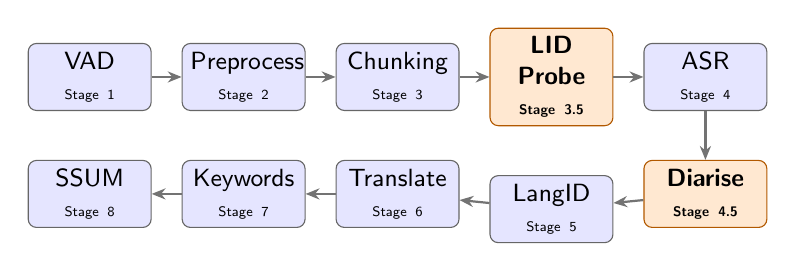
\begin{tikzpicture}[
  box/.style={draw=black!60, rectangle, rounded corners=3pt,
              fill=blue!10, font=\small\sffamily,
              text width=1.35cm, minimum height=0.65cm,
              align=center, inner sep=3pt},
  newbox/.style={draw=orange!70!black, rectangle, rounded corners=3pt,
                 fill=orange!18, font=\small\sffamily\bfseries,
                 text width=1.35cm, minimum height=0.65cm,
                 align=center, inner sep=3pt},
  arr/.style={-{Stealth[length=5pt,width=4pt]}, thick, draw=black!55},
  node distance=0.38cm
]
\node[box]    (n1)  {VAD\\{\tiny Stage 1}};
\node[box, right=of n1]  (n2)  {Preprocess\\{\tiny Stage 2}};
\node[box, right=of n2]  (n3)  {Chunking\\{\tiny Stage 3}};
\node[newbox, right=of n3] (n35) {LID Probe\\{\tiny Stage 3.5}};
\node[box, right=of n35] (n4)  {ASR\\{\tiny Stage 4}};

\node[newbox, below=0.62cm of n4]  (n45) {Diarise\\{\tiny Stage 4.5}};
\node[box, below=0.62cm of n35] (n5)  {LangID\\{\tiny Stage 5}};
\node[box, below=0.62cm of n3]  (n6)  {Translate\\{\tiny Stage 6}};
\node[box, below=0.62cm of n2]  (n7)  {Keywords\\{\tiny Stage 7}};
\node[box, below=0.62cm of n1]  (n8)  {SSUM\\{\tiny Stage 8}};

\draw[arr] (n1)  -- (n2);
\draw[arr] (n2)  -- (n3);
\draw[arr] (n3)  -- (n35);
\draw[arr] (n35) -- (n4);
\draw[arr] (n4)  -- (n45);
\draw[arr] (n45) -- (n5);
\draw[arr] (n5)  -- (n6);
\draw[arr] (n6)  -- (n7);
\draw[arr] (n7)  -- (n8);
\end{tikzpicture}%
}
\caption{Ten-stage processing pipeline. Novel stages (3.5 and 4.5) are highlighted in orange, addressing language misrouting and speaker attribution.}
\label{fig:pipeline}
\end{figure}

\textbf{VAD, Preprocessing, and Chunking (Stages 1--3).}
To eliminate environmental noise and channel static, Silero-VAD~\cite{silero2021vad} filters out non-speech segments. This step is critical; without it, Whisper frequently attempts to transcribe carrier hiss, generating hallucinated phrases in various languages. The signal undergoes further conditioning via a fourth-order Butterworth bandpass filter (300--3400~Hz) to isolate the human vocal range, followed by stationary spectral subtraction to eradicate static noise. Crucially, chunking occurs dynamically at speech transitions rather than fixed time intervals, preventing the truncation of initial phonemes.

\textbf{Pre-ASR Acoustic Language Probing (Stage 3.5).}
At Stage~3.5, MMS-LID-256 evaluates the preprocessed audio waveform prior to transcription. If the acoustic model identifies a language with confidence exceeding 0.65, the prediction is immediately fed to the Whisper decoder as a hard script hint. This mechanism breaks the failure loop where Whisper and text-based classifiers sequentially commit to the same incorrect language assumption. Because Stage~5 reuses these results, the MMS model is loaded only once per file, preserving memory.

\textbf{Automated Speech Transcription (Stage 4).}
The Whisper large-v3-turbo~\cite{radford2022whisper} model is executed under 8-bit integer quantisation using the CTranslate2 engine, keeping the active memory footprint under 2~GB with negligible loss in accuracy ($<$1\%)~\cite{lin2024awq}. To ensure stability, history conditioning is deactivated (\texttt{condition\_on\_previous\_text=False}) to stop infinite repetition loops triggered by channel noise. Additionally, setting the non-speech threshold to 0.70 (\texttt{no\_speech\_threshold=0.70}) prevents static from being transcribed as Portuguese or Icelandic. Beam size is fixed at 2 and temperature at 0.0 for deterministic execution.

\textbf{Low-Overhead Speaker Diarization (Stage 4.5).}
Stage~4.5 implements speaker diarization using 13 Mel-frequency cepstral coefficients, supplemented by delta and double-delta derivatives, creating a 39-dimensional feature space. These features are clustered via Ward-linkage agglomerative clustering, with the optimal speaker count $k$ dynamically selected between 1 and 4 using the within-cluster distance elbow method. Speaker tags are propagated through all downstream stages, enabling multi-speaker attribution in the final report.

\textbf{Script-Cascade and Ensemble Language Identification (Stage 5).}
Stage~5 implements a hybrid decision-making ensemble. Before initiating voting, the pipeline evaluates the Unicode properties of the generated transcript. If Gurmukhi characters (U+0A00--U+0A7F) exceed 20\%, the system overrides the ensemble and designates the language as Punjabi. Similarly, if Arabic or Nastaliq characters exceed 20\%, the candidate set is restricted to \texttt{\{ur, ks, sd, ps, fa, ar\}}. Three distinct signals are fed into the voting engine: Whisper's internal encoder-head probabilities, FastText~\cite{joulin2017bag} n-gram transcript classification, and MMS-LID-256~\cite{pratap2023scaling} raw acoustic waveform evaluation. Concordance across all three engines triggers a 10\% confidence bonus. Two-to-one majorities are resolved by averaging the agreeing pair, while complete disagreement defaults to the highest-scoring single predictor subject to a 15\% penalty. Scores below 0.60 are flagged as \texttt{uncertain}, and \texttt{LOW\_LANG\_CONFIDENCE} follows the output into every downstream stage so that the user knows which results to weigh carefully.

\textbf{Machine Translation and Downstream Analysis (Stages 6--8).}
Stage~6 manages the translation of low-resource languages. While NLLB-200-distilled-600M~\cite{costajussa2024nllb} handles most regional languages, it lacks support for Dogri (\texttt{doi}); the IndicTrans2-indic-en-1B~\cite{gala2023indictrans2} model is loaded dynamically to bridge this gap. To conserve memory, translation engines are loaded on demand and explicitly purged from RAM via garbage collection (\texttt{del model; gc.collect()}) before the next stage. Stage~7 screens the translated text against a custom threat-indicator dictionary using exact and fuzzy matching, raising alert levels from \texttt{CLEAR} to \texttt{CRITICAL}. Finally, Stage~8 compiles a structured 5\,W summary (Who, What, Where, When, Why) using deterministic rules targeting NATO callsigns, unit designators, and MGRS grid references, with an optional quantised Qwen2.5-1.5B~\cite{qwen2025} model refining the extracted parameters. All confidence flags---\texttt{LOW\_LANG\_CONFIDENCE}, \texttt{ASR\_LOW\_CONFIDENCE}, \texttt{TRANSLATION\_FAILED}, \texttt{TRANSLATION\_UNRELIABLE}---are preserved and propagated to the final output.

\section{Experimental Setup}

\textbf{Hardware:}
All experiments were conducted on a resource-constrained consumer laptop featuring an Apple M-series processor, 16~GB of unified RAM, and no active internet connectivity. Memory allocation was managed by loading models sequentially and releasing them prior to the initiation of subsequent stages. Table~\ref{tab:hw} documents the computational footprint of each stage, demonstrating that the cumulative system peak remains well within the target hardware limits.

\begin{table}[htbp]
\caption{Hardware and Software Resource Profile across Pipeline Stages}
\label{tab:hw}
\begin{center}
\scriptsize
\begin{tabular}{p{1.6cm}p{2.3cm}rr}
\toprule
\textbf{Stage} & \textbf{Model} & \textbf{Params} & \textbf{Peak RAM} \\
\midrule
VAD / Prep & Silero-VAD & --- & $<$0.2~GB \\
LID Probe (S3.5) & MMS-LID-256 & 150M & $\sim$0.6~GB \\
ASR (S4) & Whisper lv3-turbo CT2 int8 & 809M & $\sim$1.9~GB \\
Text LID & FastText lid.176.bin & --- & $\sim$0.9~GB \\
Translation & NLLB-200-dist.-600M & 600M & $\sim$2.4~GB \\
SSUM (opt.) & Qwen2.5-1.5B int4 & 1.5B & $\sim$1.1~GB \\
\midrule
\textbf{Total (peak)} & \multicolumn{3}{r}{\textbf{$<$7.8~GB --- fits a consumer laptop or desktop PC}} \\
\bottomrule
\end{tabular}
\end{center}
\end{table}

\textbf{Evaluation sets.}
\textit{(a) Qualitative cohort (14 samples):} three English clips, three Punjabi clips, two Hindi clips (one local recording and one FLEURS), and two FLEURS samples each for Urdu, Nepali, and Mandarin. Per-source breakdown in Table~\ref{tab:langid}.

\textit{(b) Integrated evaluation (180 samples):} 30 FLEURS test clips across six languages (\texttt{en\_us}, \texttt{pa\_in}, \texttt{hi\_in}, \texttt{ur\_pk}, \texttt{ne\_np}, \texttt{cmn\_hans\_cn}), clipped to 2--20~s, all ten stages active. Mandarin Chinese is included to simulate operational monitoring along critical lines of communication, not as a high-resource control. Source for Tables~\ref{tab:asr} and \ref{tab:largescale}.

\textit{(c) Ablation set (1,475 samples):} 295 FLEURS clips per language across five languages, \texttt{language\_hint=None} held constant to exclude Stage~3.5. Table~\ref{tab:ablation}.

\section{Experimental Results}

\subsection{ASR Performance}
\label{sec:asr}

Segment confidence is $\text{conf} = \min(1.0,\max(0.0,\,1 + \text{avg\_logprob}/4))$---Whisper's average token log-probability, linearly mapped from $[-4,\,0]$ to $[0,\,1]$. The Trans.\ column in Table~\ref{tab:asr} counts files that survived the no-speech filter; files that did not contributed 0.000 to the language mean.

\begin{table}[htbp]
\caption{ASR Performance by Language --- Full 10-Stage Pipeline ($N=30$ per language, FLEURS test split)}
\label{tab:asr}
\begin{center}
\begin{tabular}{lrrrl}
\toprule
\textbf{Language} & \textbf{N} & \textbf{Trans.} & \textbf{Mean Conf} & \textbf{RTF} \\
\midrule
English (en) & 30 & 29/30 & 0.855 & 2.91$\times$ \\
Punjabi (pa) & 30 & 29/30 & 0.870 & 4.57$\times$ \\
Hindi (hi)   & 30 & 30/30 & 0.879 & 4.11$\times$ \\
Urdu (ur)    & 30 & 19/30 & 0.455 & 8.98$\times$ \\
Nepali (ne)  & 30 & 8/30  & 0.187 & 7.00$\times$ \\
Mandarin (zh)& 30 & 27/30 & 0.819 & 6.40$\times$ \\
\midrule
\multicolumn{5}{p{7.5cm}}{\footnotesize RTF = total pipeline processing time / speech duration (CPU int8, all ten stages). Mean Conf includes 0.000 for non-transcribed files. Mandarin lower mean partly reflects 3 files filtered by the no-speech threshold. Whisper published WER~\cite{radford2022whisper}: en$\approx$2.7\%. Ours (Table~\ref{tab:largescale}): hi 46.2\%; ur 74.4\%.} \\
\bottomrule
\end{tabular}
\end{center}
\end{table}

The data indicate that transcription confidence correlates with the density of the training corpus. Highly represented languages such as English, Punjabi, and Hindi exhibit elevated confidence levels of 0.855, 0.870, and 0.879, respectively. Mandarin is close at 0.819, though three files were caught by the no-speech filter and pulled the mean down. Conversely, low-resource targets like Urdu and Nepali suffer from severe transcription failures, with Whisper often rejecting the input entirely. Of 30 Urdu files, only 19 survived the no-speech filter and produced transcripts; for Nepali, only 8 did. Segment confidence proved a useful proxy for downstream LangID and translation reliability, requiring no reference transcript to compute.

\subsection{Language Identification Ensemble Results}
\label{sec:langid}

Per-source predictions for all 14 samples appear in Table~\ref{tab:langid}. The ensemble dynamics are highly visible in the Punjabi cases. On \texttt{sent\_1} and \texttt{fleurs-pa-001}, Whisper and FastText both incorrectly predicted Hindi due to Devanagari transcription script bias, but MMS-LID's acoustic prediction overrode them to yield the correct Punjabi classification. However, on \texttt{cv-pa.mp3}, Whisper hallucinated Icelandic, which FastText validated, resulting in an incorrect ensemble decision where the acoustic model was outvoted. Similarly, Nepali suffered from Devanagari/Gujarati confusion, where Whisper and FastText predicted Gujarati, outvoting the correct MMS-LID prediction. English, Urdu, and Mandarin were unambiguous---all three sources agreed in every case, with Whisper remaining above 0.84 throughout.

\begin{table*}[htbp]
\caption{Three-Source LangID Results (Qualitative Set, 14 samples)}
\label{tab:langid}
\begin{center}
\small
\begin{tabular}{p{2.0cm}lp{2.0cm}p{1.6cm}p{1.6cm}l}
\toprule
\textbf{File} & \textbf{True} & \textbf{Whisper} & \textbf{FT} & \textbf{MMS} & \textbf{Final} \\
\midrule
\multicolumn{6}{l}{\footnotesize\textit{English}} \\
harvard        & en & en 0.999$\checkmark$ & en 0.867$\checkmark$ & en 0.996$\checkmark$ & \textbf{en}$\checkmark$ \\
LJ001          & en & en 1.000$\checkmark$ & en 0.991$\checkmark$ & en 0.991$\checkmark$ & \textbf{en}$\checkmark$ \\
Spkr26         & en & en 1.000$\checkmark$ & en 0.980$\checkmark$ & en 0.968$\checkmark$ & \textbf{en}$\checkmark$ \\
\midrule
\multicolumn{6}{l}{\footnotesize\textit{Punjabi: corrected by MMS-LID}} \\
sent\_1        & pa & hi 0.690$\times$ & hi 0.891$\times$ & pa 1.000$\checkmark$ & \textbf{pa}$\checkmark$ \\
fleurs-pa-001  & pa & hi 0.921$\times$ & hi 0.995$\times$ & pa 0.999$\checkmark$ & \textbf{pa}$\checkmark$ \\
\multicolumn{6}{l}{\footnotesize\textit{Punjabi: 2-vs-1 ensemble failure}} \\
cv-pa.mp3      & pa & is 0.981$\times$ & is 0.998$\times$ & pa 0.999$\checkmark$ & is$\times$ \\
\midrule
\multicolumn{6}{l}{\footnotesize\textit{Hindi}} \\
Hindi-009      & hi & hi 0.927$\checkmark$ & hi 1.000$\checkmark$ & ur 0.795$\times$ & \textbf{hi}$\checkmark$ \\
fleurs-hi-001  & hi & hi 0.831$\checkmark$ & hi 1.000$\checkmark$ & hi 0.995$\checkmark$ & \textbf{hi}$\checkmark$ \\
\midrule
\multicolumn{6}{l}{\footnotesize\textit{Urdu}} \\
fleurs-ur-001  & ur & ur 0.965$\checkmark$ & ur 0.998$\checkmark$ & ur 0.996$\checkmark$ & \textbf{ur}$\checkmark$ \\
fleurs-ur-002  & ur & ur 0.842$\checkmark$ & ur 0.969$\checkmark$ & ur 0.713$\checkmark$ & \textbf{ur}$\checkmark$ \\
\midrule
\multicolumn{6}{l}{\footnotesize\textit{Nepali: Devanagari/Gujarati confusion}} \\
fleurs-ne-001  & ne & gu 0.227$\times$ & gu 1.000$\times$ & ne 1.000$\checkmark$ & gu$\times$ \\
fleurs-ne-002  & ne & gu 0.306$\times$ & gu 1.000$\times$ & ne 1.000$\checkmark$ & gu$\times$ \\
\midrule
\multicolumn{6}{l}{\footnotesize\textit{Mandarin}} \\
fleurs-zh-001  & zh & zh 0.996$\checkmark$ & zh 0.999$\checkmark$ & zh 0.996$\checkmark$ & \textbf{zh}$\checkmark$ \\
fleurs-zh-002  & zh & zh 0.999$\checkmark$ & zh 0.888$\checkmark$ & zh 0.999$\checkmark$ & \textbf{zh}$\checkmark$ \\
\midrule
\multicolumn{6}{l}{\footnotesize $\checkmark$ = correct; $\times$ = incorrect. is = Icelandic; gu = Gujarati.} \\
\bottomrule
\end{tabular}
\end{center}
\end{table*}

\subsection{LangID Ablation Study}
\label{sec:ablation}

The ablation evaluated four configurations across 1,475 samples (295 per language, five border-region languages), with \texttt{language\_hint=None} held constant to exclude Stage~3.5 conditioning from all runs; results appear in Table~\ref{tab:ablation}.

\begin{table*}[htbp]
\caption{LangID Accuracy Ablation: Component Contribution (\%, 95\% CI, 295 samples/language, FLEURS test split, 5 languages)}
\label{tab:ablation}
\begin{center}
\scriptsize
\begin{tabular}{lcccccr}
\toprule
\textbf{Configuration} & \textbf{pa} & \textbf{hi} & \textbf{ur} & \textbf{ne} & \textbf{zh} & \textbf{Ovrl.} \\
\midrule
Whisper-only & 0.0 [0,0] & 85.1 [81,89] & 58.0 [52,63] & 0.0 [0,0] & 100.0 [100,100] & 48.6\% \\
\texttt{+}FastText & 0.0 [0,0] & 85.1 [81,89] & 57.3 [52,63] & 12.5 [9,16] & 99.3 [98,100] & 50.8\% \\
\texttt{+}MMS-LID & 91.9 [89,95] & 85.1 [81,89] & 58.0 [53,64] & 19.3 [15,24] & 99.3 [98,100] & 70.7\% \\
Full VANI & \textbf{91.2 [88,94]} & \textbf{85.1 [81,89]} & \textbf{58.0 [52,64]} & \textbf{19.3 [15,24]} & \textbf{99.3 [98,100]} & \textbf{70.6\%} \\
\midrule
\multicolumn{7}{l}{\footnotesize Punjabi (pa), Hindi (hi), Urdu (ur), Nepali (ne), Mandarin Chinese (zh). FLEURS test split.} \\
\multicolumn{7}{l}{\footnotesize CIs bootstrapped ($n$=10{,}000 resamples). \texttt{language\_hint=None} throughout; Stage~3.5 conditioning deliberately disabled to isolate each component.} \\
\bottomrule
\end{tabular}
\end{center}
\end{table*}

The ablation experiments in Table~\ref{tab:ablation} demonstrate the individual contribution of each pipeline module. Disabling the acoustic probe reveals that FastText provides only marginal benefits (+2.2~pp, 48.6\%$\rightarrow$50.8\%) because it inherits errors from incorrect transcripts. Integrating MMS-LID yields a +19.9~pp increase in macro-average accuracy (50.8\%$\rightarrow$70.7\%) because it classifies directly from the raw waveform, independent of the ASR output.

For Punjabi, the impact of acoustic modelling is binary: accuracy rises from 0.0\% (where every sample is misrouted as Hindi) to 91.9\% (CI [89--95\%]). Nepali rises to 19.3\%, reflecting the limitations of Whisper's baseline transcription quality on Nepali audio. Urdu was flat across all four ablation rows (57--58\%) because, without a language hint, Whisper writes Urdu audio in Devanagari and the Arabic-script filter finds nothing to act on. Supplying \texttt{language\_hint=ur} via Stage~3.5 in the integrated run switches the output to Nastaliq and lifts Urdu identification accuracy to 70.0\%---a 12~pp gain attributable to the pre-ASR conditioning loop, not the ensemble itself.

\subsection{Integrated Pipeline Evaluation}
\label{sec:largescale}

The aggregate performance metrics of the fully integrated pipeline are presented in Table~\ref{tab:largescale}, demonstrating high identification accuracy for Hindi and Punjabi. English LangID was 30/30 and Mandarin 29/30 (conf/RTF in Table~\ref{tab:asr}; counts exceed Trans.\ as Stage~3.5 runs before ASR); the single Mandarin miss was a \texttt{zh-tw}/\texttt{zh} label mismatch.

\begin{table*}[htbp]
\caption{Aggregate Integrated Pipeline Performance (30 FLEURS Samples per Language)}
\label{tab:largescale}
\begin{center}
\begin{tabular}{lllll}
\toprule
\textbf{Metric} & \textbf{Punjabi (pa)} & \textbf{Hindi (hi)} & \textbf{Urdu (ur)} & \textbf{Nepali (ne)} \\
\midrule
LangID accuracy & \textbf{29/30 (96.7\%)} & \textbf{29/30 (96.7\%)} & 21/30 (70.0\%) & 19/30 (63.3\%) \\
Mean WER & N/A$^\dagger$ & \textbf{46.2\%} & 74.4\% & N/A$^\ddagger$ \\
Mean CER & N/A$^\dagger$ & \textbf{32.4\%} & 63.2\% & N/A$^\ddagger$ \\
Mean seg.\ confidence & 0.870 & \textbf{0.879} & 0.455 & 0.187 \\
Mean RTF (CPU) & 4.57$\times$ & 4.11$\times$ & 8.98$\times$ & 7.00$\times$ \\
Trans.\ stage (30/30) & 100\% & 100\% & 100\% & 100\% \\
\midrule
\multicolumn{5}{l}{\footnotesize $^\dagger$ Non-comparable: Whisper outputs Devanagari for Punjabi; FLEURS references are in Gurmukhi script.} \\
\multicolumn{5}{l}{\footnotesize $^\ddagger$ Non-comparable: Whisper hallucinated European-language text on low-confidence Nepali audio (mean conf.\ 0.187).} \\
\bottomrule
\end{tabular}
\end{center}
\end{table*}

The 96.7\% accuracy for Hindi and Punjabi represents a significant improvement over the 35.8\% Whisper-only baseline (Table~\ref{tab:baselines}). One failure in each language arose from audio containing heavy Urdu/Persian loanwords that shifted the ensemble toward Urdu. Urdu's 70.0\% accuracy depends heavily on Stage~3.5's pre-ASR script hint; without it, Whisper writes Urdu in Devanagari script, which bypasses the Nastaliq character filter. The 11 Nepali failures are Whisper hallucinations---European text on low-confidence audio (mean conf.\ 0.187)---with MMS-LID voting correctly in four of those cases but being overruled each time.

\subsection{Translation and SSUM}
\label{sec:trans}

Translation executed successfully across all 120 Indic files (pa/hi/ur/ne), showing that while poor transcription degrades translation quality, it does not prevent the pipeline from completing. Hindi cascade translation metrics appear in Table~\ref{tab:bleu}, and Table~\ref{tab:isum_example} illustrates the structured intelligence output generated from a Punjabi audio segment; confidence flags, when raised, propagate through all downstream stages.

\begin{table}[htbp]
\caption{Hindi Cascade ASR+MT Translation Quality (30 Samples)}
\label{tab:bleu}
\begin{center}
\begin{tabular}{lrl}
\toprule
\textbf{Metric} & \textbf{Score} & \textbf{Note} \\
\midrule
Cascade BLEU & 23.5 & moderate degradation vs.\ MT ceiling \\
Cascade chrF2 & 46.4 & character-level overlap \\
Translation completion  & 100\% & 30/30 samples \\
Mean ASR WER            & 46.2\% & Hindi references \\
\bottomrule
\end{tabular}
\end{center}
\end{table}

\begin{table}[htbp]
\caption{SSUM Output: \texttt{sent\_1.wav} (Punjabi, 7.0~s)}
\label{tab:isum_example}
\begin{center}
\begin{tabular}{p{1.5cm}p{5.8cm}}
\toprule
\textbf{Field} & \textbf{Extracted Value} \\
\midrule
Language   & \texttt{pa} (conf 0.993, \textit{hi}$\rightarrow$\textit{pa} override) \\
\textit{Who}   & Mukhi (SPEAKER\_0), National Council NCVAT$^*$ \\
\textit{What}  & Decision to establish National Council NCVAT$^*$ \\
\textit{Where} & Not identified \\
\textit{When}  & Not identified \\
Alert level    & \texttt{CLEAR} \\
Flags          & None \\
\midrule
\multicolumn{2}{l}{\footnotesize $^*$Extracted verbatim; expansion unresolved.} \\
\bottomrule
\end{tabular}
\end{center}
\end{table}

\subsection{Robustness under Channel Degradations}
\label{sec:robustness}

The same 120 Indic samples (pa/hi/ur/ne, 30 each) ran through all four configurations under five channel conditions: clean; 300--3400~Hz bandpass; AWGN at 10~dB and 0~dB SNR; and MP3 at 16~kbps. Table~\ref{tab:robustness} has the breakdown.

\begin{table}[htbp]
\caption{Overall LangID Accuracy (\%) under Channel Degradations}
\label{tab:robustness}
\begin{center}
\begin{tabular}{lrrrr}
\toprule
\textbf{Condition} & \textbf{W} & \textbf{+FT} & \textbf{+MMS} & \textbf{Full} \\
\midrule
Clean          & 38.3 & 40.0 & 53.3 & \textbf{69.2} \\
Bandpass       & 30.0 & 30.0 & 42.5 & \textbf{54.2} \\
AWGN 10~dB     & 35.8 & 40.8 & 55.8 & \textbf{70.8} \\
AWGN 0~dB      & 22.5 & 22.5 & 30.8 & \textbf{42.5} \\
MP3 16~kbps    & 28.3 & 28.3 & 41.7 & \textbf{52.5} \\
\midrule
\multicolumn{5}{p{8cm}}{\footnotesize pa/hi/ur/ne; 30 samples each. \texttt{language\_hint=None}; W = Whisper-only. Audio was degraded offline before the pipeline.} \\
\bottomrule
\end{tabular}
\end{center}
\end{table}

As shown in Table~\ref{tab:robustness}, the acoustic-grounded ensemble consistently outperforms the text-only baseline across all noise profiles, adding +8 to +15~pp (MMS-LID contribution) over the text-only (+FastText) baseline in every condition. Under extreme bandpass and MP3 compression, text-only classification gains collapse entirely because transcription degradation destroys lexical cues; FastText gained exactly zero over Whisper-only in both conditions. In contrast, acoustic waveform modelling preserves identification capability even at 0~dB SNR, where the full pipeline reached 42.5\% against 22.5\% for Whisper-only, with no rank reversals anywhere in the table.

\subsection{Comparison with Published Baselines}

\begin{table}[htbp]
\caption{LangID Comparison with Published and Internal Baselines}
\label{tab:baselines}
\begin{center}
\begin{tabular}{llll}
\toprule
\textbf{System} & \textbf{Modal.} & \textbf{Langs} & \textbf{Accuracy} \\
\midrule
\multicolumn{4}{p{8cm}}{\footnotesize\textit{Published figures: clean, balanced, general-domain benchmarks}} \\
FastText~\cite{joulin2017bag} & Text & 176--217 & $>$97\% \\
MMS-LID~\cite{pratap2023scaling} & Audio & 256 & $>$90\% \\
Whisper~\cite{radford2022whisper} & A+T & 99 & $\sim$95\% \\
\midrule
\multicolumn{4}{p{8cm}}{\footnotesize\textit{Ours: integrated pipeline, 180 samples, border-region languages}} \\
Whisper-only (internal) & A+T & 4 & 35.8\%$^\dagger$ \\
Full VANI Ensemble & A+T & 4 & \textbf{81.7\%}$^\ddagger$ \\
\multicolumn{4}{p{7.5cm}}{\footnotesize $^\dagger$ Macro-average for pa/hi/ur/ne from ablation (Table~\ref{tab:ablation}): $(0+85.1+58.0+0)/4 = 35.8\%$, \texttt{language\_hint=None}.} \\
\multicolumn{4}{p{7.5cm}}{\footnotesize $^\ddagger$ Macro-average for pa/hi/ur/ne from Table~\ref{tab:largescale}: $(96.7+96.7+70.0+63.3)/4 = 81.7\%$.} \\
\bottomrule
\end{tabular}
\end{center}
\end{table}

Table~\ref{tab:baselines} compares the VANI pipeline to established baseline models, illustrating the impact of the targeted border-region test set on standard evaluation metrics. Published Whisper achieves $\sim$95\% on balanced general-domain benchmarks; our Whisper-only baseline reaches only 35.8\% on this test set. The $\sim$59~pp gap is not a contradiction---it is the test set. Punjabi and Nepali both approach zero under Whisper-only and are included precisely because they represent the operationally critical languages in this domain.

\section{Discussion}

The high error rate of standard speech recognition models on regional languages is primarily driven by unbalanced training datasets. Whisper's training corpus contains several orders of magnitude more Hindi than Punjabi, leading the model to default to Hindi when processing phonologically similar Punjabi audio. This bias propagates to text-based classifiers like FastText, which accept the incorrect Devanagari transcript and validate the wrong language. On \texttt{sent\_1.wav}, Whisper returned Hindi at 0.690 and FastText agreed at 0.891---both wrong. MMS-LID returned Punjabi at 1.000, and the Gurmukhi script-cascade override in Stage~5 corrected the ensemble, a mechanism that requires MMS-LID to have first identified the language acoustically. By incorporating raw waveform classification at Stage~3.5, the pipeline breaks this failure loop, demonstrating that robust multilingual processing requires acoustic validation independent of the ASR output.

Remaining limitations stem from specific linguistic and script features. Urdu accuracy is highly dependent on Stage~3.5 providing a Nastaliq script hint; without it, Devanagari output bypasses the Arabic/Nastaliq filter entirely. Nepali and Hindi share the Devanagari script, making Unicode character filtering ineffective for disambiguation; integrating morphological checks targeting Nepali postpositions represents the most direct path to improvement without modifying any acoustic model. Mandarin Chinese is correctly identified in 99.3\% (CI [98--100\%]) of test cases without any pre-transcription hint---the one failure being a \texttt{zh-tw}/\texttt{zh} label mismatch resolvable with a one-line alias table. FLEURS is read speech; conversational registers, code-switching, and regional varieties remain untested. RTF of 3--9$\times$ on CPU suits post-collection batch work; GPU deployment drops that below 0.3$\times$.

\section{Conclusion}

This study demonstrates that offline language identification and translation for low-resource regional languages can be successfully executed on standard consumer-grade hardware. The primary requirement for preventing silent transcription failures is that the system must draw on classification signals beyond the raw ASR transcript. The experimental findings confirm this: incorporating an acoustic waveform classifier improved macro-average language identification accuracy by 19.9 percentage points and raised Punjabi identification from 0.0\% to 91.9\%.

Urdu and Nepali sit at 70.0\% and 63.3\%, and neither gap is opaque. Urdu's number depends on Stage~3.5 delivering Nastaliq output; without it the Arabic-script filter is blind. Nepali shares a script with Hindi, so character counts contribute nothing; Nepali-specific morphology is the obvious next lever. Bengali, Pashto, and code-switched field recordings are the next evaluation targets, together with a diarization run against annotated multispeaker material.

\begin{thebibliography}{99}

\bibitem{radford2022whisper} A. Radford et al., ``Robust speech recognition via large-scale weak supervision,'' in \textit{Proc. 40th Int.\ Conf.\ Machine Learning (ICML)}, Honolulu, HI, 2023. doi: 10.48550/arxiv.2212.04356.

\bibitem{pratap2023scaling} V. Pratap et al., ``Scaling speech technology to 1,000+ languages,'' in \textit{Proc. 37th Conf.\ Neural Information Processing Systems (NeurIPS)}, New Orleans, LA, 2023. doi: 10.48550/arxiv.2305.13516.

\bibitem{costajussa2024nllb} M. R. Costa-juss\`a et al., ``Scaling neural machine translation to 200 languages,'' \textit{Nature}, vol.~630, pp.~841--846, 2024. doi: 10.1038/s41586-024-07335-x.

\bibitem{barrault2023seamless} L. Barrault et al., ``SeamlessM4T: Massively Multilingual \& Multimodal Machine Translation,'' \textit{arXiv preprint arXiv:2308.11596}, 2023. doi: 10.48550/arxiv.2308.11596.

\bibitem{conneau2023fleurs} A. Conneau et al., ``FLEURS: Few-shot learning evaluation of universal representations of speech,'' in \textit{Proc. IEEE Spoken Language Technology Workshop (SLT)}, 2023. doi: 10.48550/arxiv.2205.12446.

\bibitem{joulin2017bag} A. Joulin et al., ``Bag of tricks for efficient text classification,'' in \textit{Proc. 15th Conf.\ European Chapter of the ACL (EACL)}, Valencia, Spain, Apr.\ 2017, pp.~427--431. doi: 10.48550/arxiv.1607.01759.

\bibitem{qwen2025} Qwen Team, ``Qwen2.5 Technical Report,'' \textit{arXiv preprint arXiv:2412.15115}, 2024. doi: 10.48550/arxiv.2412.15115.

\bibitem{gala2023indictrans2} J. Gala et al., ``IndicTrans2: Towards high-quality and accessible machine translation models for all 22 scheduled Indian languages,'' \textit{Trans.\ Machine Learning Research}, 2023. doi: 10.48550/arxiv.2305.16307.

\bibitem{gandhi2023distilwhisper} S. Gandhi, P. von Platen, and A. M. Rush, ``Distil-Whisper: Robust knowledge distillation via large-scale pseudo labelling,'' \textit{arXiv preprint arXiv:2311.00430}, 2023. doi: 10.48550/arxiv.2311.00430.

\bibitem{plaquet2023powerset} A. Plaquet and H. Bredin, ``Powerset multi-class cross entropy loss for neural speaker diarization,'' in \textit{Proc. INTERSPEECH}, Dublin, 2023, pp.~3500--3504. doi: 10.21437/interspeech.2023-205.

\bibitem{lin2024awq} J. Lin et al., ``AWQ: Activation-aware weight quantization for on-device LLM compression and acceleration,'' in \textit{Proc. Machine Learning and Systems (MLSys)}, Santa Clara, CA, 2024. doi: 10.1145/3714983.3714987.

\bibitem{silero2021vad} Silero Team, ``Silero VAD: pre-trained enterprise-grade Voice Activity Detector,'' GitHub, 2021. [Online]. Available: \url{https://github.com/snakers4/silero-vad}

\end{thebibliography}

\end{document}
